\section{Arquitectura del código}

El proyecto se compone de \textbf{tres versiones} del mismo programa, más una serie de módulos compartidos y los scripts que automatizan el experimento. La figura~\ref{fig:estructura} muestra el árbol completo de archivos.

\begin{figure}[H]
    \centering
    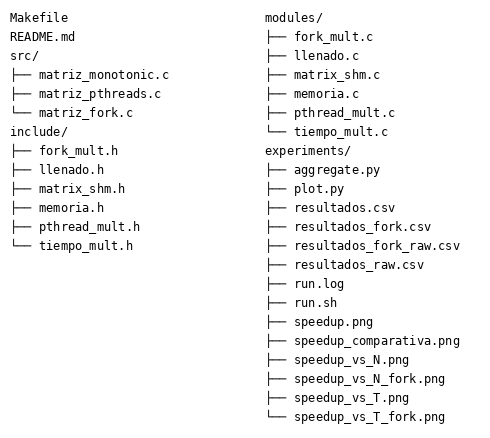
\includegraphics[width=0.95\textwidth]{figuras/estructura_proyecto.png}
    \caption{Estructura de carpetas y archivos del proyecto.}
    \label{fig:estructura}
\end{figure}

\subsection{Versión secuencial}

Es el programa base sobre el que se construyen las versiones paralelas. Recibe como argumentos el tamaño de la matriz \texttt{N} y un valor máximo, reserva memoria para tres matrices, las llena con números aleatorios, ejecuta el triple bucle de multiplicación y mide el tiempo. El código vive en \texttt{src/matriz\_monotonic.c}.

\subsection{Versión con pthreads}

Variante que reparte las filas de la matriz resultado entre varios hilos usando la API POSIX Threads. Los hilos se crean con \texttt{pthread\_create} y el programa principal espera con \texttt{pthread\_join}. El código de la paralelización vive en \texttt{modules/pthread\_mult.c}.

\subsection{Versión con fork y memoria compartida}

Variante que crea procesos con \texttt{fork()} en lugar de hilos. Como cada proceso tiene su propio espacio de direcciones, las matrices se crean en \textbf{memoria compartida POSIX} para que padre e hijos vean los mismos datos. El padre espera a cada hijo con \texttt{waitpid()}. El código de la paralelización vive en \texttt{modules/fork\_mult.c} y la gestión de la memoria compartida en \texttt{modules/matrix\_shm.c}.

\subsection{Estrategia de partición}

Las tres versiones paralelas usan la \textbf{misma estrategia}: repartir las filas de la matriz resultado $C$ entre los trabajadores. Cada uno calcula las filas que le corresponden y solo escribe en esa parte, así que no hay conflicto entre ellos.

El reparto es equitativo: si $N$ es divisible por la cantidad de hilos/procesos, cada uno recibe $N/T$ filas. Si no, los primeros reciben una fila extra para balancear la carga. El siguiente ejemplo muestra la partición para $N = 1000$ y $T = 4$:

\begin{center}
\begin{tabular}{|c|c|}
\hline
\textbf{Hilo / Proceso} & \textbf{Filas asignadas} \\
\hline
0 & $[0, 250)$ \\
1 & $[250, 500)$ \\
2 & $[500, 750)$ \\
3 & $[750, 1000)$ \\
\hline
\end{tabular}
\end{center}

\subsection{Por qué no se necesita sincronización adicional}

Como cada hilo o proceso escribe \textbf{exclusivamente} en su propio rango de filas de la matriz $C$, no hay condiciones de carrera: dos trabajadores nunca escriben sobre la misma posición. Los trabajadores leen de $A$ y $B$ sin escribir, lo cual es seguro. La única sincronización necesaria es al final: \texttt{pthread\_join} en la versión pthreads, o \texttt{waitpid} en la versión fork, para que el programa principal espere a que todos terminen antes de mostrar el resultado.
